\documentclass{article}
\usepackage[utf8]{inputenc}
\usepackage{amsmath}\usepackage{setspace}
\usepackage{graphicx} 
\usepackage{amssymb}
\usepackage{amsthm}
\usepackage{listings}
\usepackage{xcolor}
\usepackage{color}
\definecolor{yellow}{rgb}{0.99,0.97,0.89}
\pagecolor{yellow}
\usepackage{indentfirst} 
\usepackage{natbib}
\usepackage{verbatim}
\usepackage{indentfirst}
\usepackage[all,cmtip]{xy}
\usepackage{tikz-cd}
\usepackage[colorlinks,linkcolor=blue]{hyperref}

\newtheorem{theorem}{Theorem}[section]
\newtheorem{lemma}[theorem]{Lemma}
\newtheorem*{claim}{Claim}
\newtheorem{corollary}[theorem]{Corollary}
\theoremstyle{definition}
\newtheorem{definition}[theorem]{Definition}
\newtheorem{example}[theorem]{Example}
\newtheorem{xca}[theorem]{Exercise}
\newtheorem{proposition}[theorem]{Proposition}
\theoremstyle{remark}
\newtheorem{remark}[theorem]{Remark}

\numberwithin{equation}{section}


%\newtheorem{example}{Example}[section]              
\newtheorem{algorithm}{Algorithm}
%\newtheorem{theorem}{Theorem}[section]  
%\newtheorem{definition}{Definition}[section]  
\newtheorem{axiom}{Axiom}
\newtheorem{property}{Property}

%\newtheorem{lemma}{Lemma}
%\newtheorem{corollary}{Corollary}[section]  
%\newtheorem{remark}{Remark}[section] 
\newtheorem{condition}{Condition}
\newtheorem{conclusion}{Conclusion}
\newtheorem{assumption}{Assumption}

\begin{document}
\title{The Homology of $SL_2(\mathbb{Z})$}
\author{Wei Yunsong}
\date{June 2020}


\setlength{\parindent}{2em}
\maketitle
\tableofcontents
\newpage
\section{Introduction}
This is a note written for the final project of the course Group Cohomology. In this note I state how to calculate the homology of $SL_2(\mathbb{Z})$. 
\par
To begin with, I define what is the homology $H_\ast G$ of a group G in chapter \ref{chap2.1} and then show that this is equal to the homology of the K(G,1)-complex in theorem \ref{thm1}.  Using the Seifert-van Kampen theorem. I proved the Whitehead theorem \ref{thm2}, which says the functor $K(-, 1)$ preserves push-out, and so I get the Mayor-Vietoris sequence for homology of the amalgamation product $G=G_{1} *_{A} G_{2}$(corollary \ref{cor1}).
\par
Later, I show in chapter \ref{chap3} that the group action on a tree somehow determined the group. Especially, I proved theorem \ref{thm3.3} that when a group G acts without inversions on a tree in such a way that $G$ acts transitively on edges, then G can be presented as amalgamations. Luckily, the group action of $SL_2(\mathbb{Z})$ on the Farey Tree defined in chapter \ref{chap4.1} is proved to have such properties(chapter \ref{chap4.2}), and thus $S L_{2}(\mathbb{Z}) \cong \mathbb{Z} / 4 *_{\mathbb{Z} / 2} \mathbb{Z} / 6$(theorem \ref{thmain}) being shown. 
\par
Finally, by computing the Mayor-Vietoris sequence for homology of the amalgamation product of $S L_{2}(\mathbb{Z}) \cong \mathbb{Z} / 4 *_{\mathbb{Z} / 2} \mathbb{Z} / 6$, the homology of $S L_{2}(\mathbb{Z})$ is obtained(theorem \ref{thm3}).
\section{The Homology of a Group}
\subsection{The Definition of $H_\ast G$}
\label{chap2.1}
\begin{definition}
Let $G$ be a group and $\varepsilon: F \rightarrow \mathbb{Z}$ a projective resolution of $\mathbb{Z}$ over $\mathbb{Z} G$. We define the homology groups of $G$ by
\[
H_{i} G=H_{i}\left(F_{G}\right)
\]
where $M_{G}=M\otimes_{\mathbb{Z}G}\mathbb{Z}$ is the group of co-invariants of a $G$-module $M$.
\end{definition}
We need to examine that the right-hand side is independent of the choice of resolution, up to canonical isomorphism. 
\begin{theorem}
Given projective resolutions $F$ and $F^{\prime}$ of a module $M,$ there is an augmentation-preserving chain map $f: F \rightarrow F^{\prime},$ unique up to homotopy, and $f$
is a homotopy equivalence.
\end{theorem}
\begin{proof}
See \cite{brown2012cohomology}cf.I(7.5)
\end{proof}

Therefore we can compute the homology of a group via any resolution. 

\begin{example}
\label{example1}
suppose $G$ is a finite cyclic group of order $n$. Using the resolution
\[
\ldots \stackrel{t-1}{\longrightarrow} \mathbb{Z} G \stackrel{N}{\rightarrow} \mathbb{Z} G \stackrel{t-1}{\longrightarrow} \mathbb{Z} G \rightarrow \mathbb{Z} \rightarrow 0
\]
We obtain the complex
\[
\cdots \stackrel{0}{\rightarrow} \mathbb{Z} \stackrel{n}{\rightarrow} \mathbb{Z} \stackrel{0}{\rightarrow} \mathbb{Z}
\]
Thus
\[
H_{i} G \simeq \left\{\begin{array}{ll}
\mathbb{Z} & i=0 \\
\mathbb{Z}_{n} & i \text { odd } \\
0 & i \text { even }
\end{array}\right.
\]
\end{example}

\subsection{Topological Interpretation}
Via the complex of $K(G,1)$ space we can get a free resolution over $\mathbb{Z}G$. We will prove the following in this section:
\begin{theorem}
\label{thm1}
If $Y$ is a $K(G,1)$-complex then $H_\ast G\simeq H_\ast Y $
\end{theorem}
We begin with some definitions
\begin{definition}
By a $G$-complex we will mean a CW-complex X together with an action of G on X which permutes the cells.
\end{definition}
Thus we have for each $g \in G$ a homeomorphism $x \mapsto g x$ of $X$ such that the image $g \sigma$ of any cell $\sigma$ of $X$ is again a cell. For example, if $X$ is a simplicial complex on which $G$ acts simplicially, then $X$ is a $G$-complex.
\par
If $X$ is a $G$-complex then the action of $G$ on $X$ induces an action of $G$ on the cellular chain complex $C_{*}(X),$ which thereby becomes a chain complex of $G$ -modules. Moreover, the canonical augmentation $\varepsilon: C_{0}(X) \rightarrow \mathbb{Z}$ (defined by $\varepsilon(v)=1$ for every 0 -cell $v$ of $X$ ) is a map of $G$ -modules.
\par
\begin{definition}
$X$ is a free $G$-complex if the action of $G$ freely permutes the cells of $X$ (i.e., $g \sigma \neq \sigma$ for all $\sigma$ if $g \neq 1$ ). 
\end{definition}
In this case each chain module $C_{n}(X)$ has a $\mathbb{Z}$ -basis which is freely permuted by $G,$ hence $ C_{n}(X)$ is a free $\mathbb{Z} G$ -module with one basis element for every $G$-orbit of cells. 
\par
Finally, if $X$ is contractible, then $H_{*}(X) \approx H_{*}(\mathrm{pt} .) ;$ in other words, the sequence
\[
\cdots \rightarrow C_{n}(X) \stackrel{\partial}{\rightarrow} C_{n-1}(X) \rightarrow \cdots \rightarrow C_{0}(X) \stackrel{\varepsilon}{\rightarrow} \mathbb{Z} \rightarrow 0
\]
is exact. We have, therefore:
\begin{proposition}
\label{prop1}
Let $X$ be a contractible free $G$-complex. Then the augmented cellular chain complex of $X$ is a free resolution of $\mathbb{Z}$ over $\mathbb{Z} G$
\end{proposition}
If $Y$ is a $K(G, 1)$ then the universal cover $p: X \rightarrow Y$ is a regular cover(i.e. the deck transformations act transitively on the fibre) whose group of deck transformations is isomorphic to $\pi_{1} Y=G$.  We therefore obtain from proposition \ref{prop1}:
\begin{proposition}
If $Y$ is a $K(G, 1)$ then the augmented cellular chain complex of the universal cover of $Y$ is a free resolution of $\mathbb{Z}$ over $\mathbb{Z} G$
\end{proposition}
Now we move to the key lemma:
\begin{lemma}
Let $X$ be a free $G$-complex and let $Y$ be the orbit complex
$X / G .$ Then $C_{*}(Y) \approx C_{*}(X)_{G}$.
\end{lemma}
\begin{proof}
The projection $C_{*}(X) \rightarrow C_{*}(Y)$ induces by passage to the quotient $\operatorname{arap} \varphi: C_{*}(X)_{G} \rightarrow C_{*}(Y) .$ Now $C_{*}(X)_{G}$ has a $\mathbb{Z}$-basis with one basis element for each $G$-orbit of cells of $X$(According to the definition, If $F$ is a free $\mathbb{Z} G$ -module with basis $\left(e_{i}\right),$ then $F_{G}$ is a free $\mathbb{Z}$-module with basis $\left(\bar{e}_{i}\right)$). But $C_{*}(Y)$ also has a $\mathbb{Z}$ -basis with one element for each $G$-orbit of cells of $X,$ and it is clear that $\varphi$ maps a basis element of $C_{*}(X)_{G}$ to the corresponding basis element of $C_{*}(Y),$ hence $\varphi$ is an isomorphism.
\end{proof}
Let X be the universal cover of Y, the $K(G,1)$-complex, then we have $C_{*}(Y) \approx C_{*}(X)_{G}$ and thus proved the theorem \ref{thm1}.

\newpage
\subsection{The Homology of Amalgamated Free Products}
\begin{definition}
Suppose we are given groups $G_{1}, G_{2},$ and $A$ and homomorphisms $\alpha_{1}:$ $A \rightarrow G_{1}$ and $\alpha_{2}: A \rightarrow G_{2} .$ By the amalgamated free product (or amalgamated sum, or amalgam) of $G_{1}$ and $G_{2}$ along $A$ we mean a group $G$ which fits into a commutative square
\begin{equation}
\label{sq}
\xymatrix{
A \ar[d]^{\alpha_1} \ar[r]^{\alpha_2} &G_2 \ar[d]^{\beta_2}\\
G_1\ar[r]^{\beta_1} & G}
\end{equation}
\par
with the following universal mapping property: Given a group $H$ and homomorphisms $\gamma_{i}: G_{i} \rightarrow H(i=1,2)$ with $\gamma_{1} \alpha_{1}=\gamma_{2} \alpha_{2},$ there is a unique map
$\varphi: G \rightarrow H$ such that $\varphi \beta_{i}=\gamma_{i} .$ We write $G=G_{1} *_{A} G_{2},$ and we say that the square \eqref{sq} is an amalgamation diagram.
\end{definition}

The universal property above shows that amalgamation is the group theoretic analogue of pasting two topological spaces together along a common subspace. The Seifert-van Kampen theorem, which the reader has probably seen in some form, makes the analogy precise via the $\pi_{1}$-functor. We will need the following simple version of that theorem:
\begin{theorem}
\label{thm_van}
Let $X$ be a $C W$-complex which is the union of two connected subcomplexes $X_{1}$ and $X_{2}$ whose intersection $Y$ is connected and non-empty.
Then the square
$$
\xymatrix{
\pi_1 Y \ar[d] \ar[r] &\pi_1 X_2\ar[d]\\
\pi_1 X_1\ar[r] & \pi_1 X}
$$
is an amalgamation diagram, where all fundamental groups are computed at a fixed vertex $y \in Y$ and all maps are induced by inclusions. Thus
\[
\pi_{1} X=\pi_{1} X_{1} *_{\pi_{1}Y} \pi_{1} X_{2}
\]
\end{theorem}
\begin{proof}
See \cite{cohen1989combinatorial}, cf.4.2, theorem 4.
\end{proof}
We can express this theorem more concisely by saying that the functor
$$\pi_{1}:(\text { connected, pointed complexes }) \rightarrow(\text { groups })$$
preserves amalgamations. In order to study the homology of amalgamations of groups, we would like to have a result going in the other direction, saying that the "functor" $K(-, 1):(\text { groups }) \rightarrow($ complexes) preserves amalgamations. This turns out to be true as long as the maps $\alpha_{1}$ and $\alpha_{2}$ of \eqref{sq} are injective:

\begin{theorem}\label{thm2}{(Whitehead)}. 

Any amalgamation diagram \eqref{sq} with $\alpha_{1}$ and $\alpha_{2}$ injective can be realized by a diagram
$$
\xymatrix{
Y \ar@{^{(}->}[d] \ar@{^{(}->}[r] &X_2\ar@{^{(}->}[d]\\
 X_1\ar@{^{(}->}[r] & X}
$$
of $K(\pi, 1)-$complexes such that $X=X_{1} \cup X_{2}$ and $Y=X_{1} \cap X_{2}$.
\end{theorem}

The proof will require three elementary lemmas:
\begin{Lemma}
\label{lemma1}
If $\alpha_{1}$ and $\alpha_{2}$ are injective then so are $\beta_{1}$ and $\beta_{2} .$ Thus $G_{1}, G_{2},$ and $A$ can be regarded as subgroups of $G$.
\end{Lemma}
\begin{proof}
See, \cite{lyndon2015combinatorial}, cf.IV.2, theorem 2.6.
\end{proof}
\begin{lemma}
\label{lemma2}
Let $X^{\prime}\hookrightarrow X$ be an inclusion of connected $C W$-complexes such that the induced map $\pi^{\prime} \rightarrow \pi$ of fundamental groups is injective. Let $p: \widetilde{X} \rightarrow X$ be the universal cover of $X .$ Then each connected component of $p^{-1} X^{\prime}$ is simply connected (hence it is a copy of the universal cover of $X^{\prime}$ ). Moreover, these components are permuted transitively by the action of $\pi$ on $\widetilde{X}$, and $\pi^{\prime}$ is the isotropy group of one of them; in other words, $\pi_{0}\left(p^{-1} X^{\prime}\right) \approx \pi / \pi^{\prime}$.
\end{lemma}
\begin{proof}
For any basepoint in $p^{-1} X^{\prime}$ we have a diagram
$$
\xymatrix{
\pi_1 (p^{-1}X^{\prime}) \ar@{^{(}->}[d] \ar[r] &\pi_1 \widetilde{X}\ar@{^{(}->}[d]\\
\pi^{\prime} \ar@{^{(}->}[r] & \pi}
$$
where the vertical maps are induced by $p$ and the horizontal maps by inclusions. since $\pi_{1} \tilde{X}=\{1\},$ the first assertion follows at once. From the definition of the action given by the fundamental group of the base space on the cover we obtain the second assertion.
\end{proof}

\begin{lemma}
\label{lemma3}
Any diagram $G_{1} \leftarrow A \rightarrow G_{2}$ of groups can be realized by a $\operatorname{diagram} X_{1} \hookleftarrow  Y \hookrightarrow X_{2}$ of $K(\pi, 1)$-complexes.
\end{lemma}
\begin{proof}
Since $\mathrm{K}(\pi, 1)$-complexes can be constructed functorially, We can therefore realize the group homomorphisms by cellular maps $X_{1} \leftarrow Y \rightarrow X_{2}$ of $K(\pi, 1)$ 's. Taking mapping cylinders if necessary as in the appendix \ref{inc}, we can make these maps inclusions.
\end{proof}

\begin{proof}
Now we can prove theorem \ref{thm2}. Start with $\operatorname{diagram} X_{1} \hookleftarrow  Y \hookrightarrow X_{2}$ as in the above lemma \ref{lemma3} and form the adjunction space $X=X_{1} \cup_{Y} X_{2},$ i.e., $X$ is obtained from the disjoint union $X_{1} \coprod X_{2}$ by identifying the two copies of $Y .$ Then $\pi_{1} X=G_{1} *_{A} G_{2}=G$ by theorem \ref{thm_van}. so we need only show that the universal cover $\tilde{X}$ satisfies $H_{i} \tilde{X}=0$ for $i>1 .$ Let $\tilde{X}_{1}, \tilde{X}_{2}$ and $\tilde{Y}$ be the inverse images of $X_{1}, X_{2},$ and $Y$ in $\tilde{X}$. since $X_{1}, X_{2},$ and $Y$ have acyclic universal covers, it follows from \ref{lemma1} and \ref{lemma2} that $\tilde{X}_{1}, \tilde{X}_{2},$ and $\tilde{Y}$ have trivial homology in positive dimensions. The Mayer-Vietoris sequence associated to the square
$$
\xymatrix{
\widetilde{Y}\ar@{^{(}->}[d] \ar@{^{(}->}[r] &\widetilde{X}_2\ar@{^{(}->}[d]\\
 \widetilde{X}_1\ar@{^{(}->}[r] & \widetilde{X}}
$$
therefore shows that $H_{i} \tilde{X}=0$ for $i>1$
\end{proof}
\begin{corollary}
\label{cor1}
Given $G=G_{1} *_{A} G_{2}$ where $A \subseteq G_{1}$ and $A\subseteq G_{2},$ there is $a$ "Mayer-Vietoris" sequence
\[
\cdots \rightarrow H_{n} A \rightarrow H_{n} G_{1} \oplus H_{n} G_{2} \rightarrow H_{n} G \rightarrow H_{n-1} A \rightarrow \cdots
\]
\end{corollary}
\begin{proof}
This is immediate from theorem \ref{thm1} and the theorem \ref{thm2}.
\end{proof}



\section{Group Action on a Tree}
\label{chap3}
A group action on a graph is a group action on the sets of vertices and edges that respects the edge
relations. We show in this chapter that the group action on a tree somehow determined the group.

\subsection{Free Actions on Trees}
We prove in this section the following theorem.
\begin{theorem}
\label{3.1}
If a group \textit{G} acts freely on a tree, then \textit{G} is isomorphic to a free group.
\end{theorem}
Our proof of this theorem has three steps. First we find a tiling of the tree that is consistent with the action of $G,$ then we use the tiling to find a generating set for $G,$ and finally we show that the generating set is a free generating set.
\par\noindent
\textbf{Step 1: Tiling the tree. }Again, the key to the proof is a certain tiling of our tree
$T .$ By a tile, we mean a subtree $T_{0}$ of the barycentric subdivision $T^{\prime}$ of $T$ (the barycentric subdivision of a graph is the graph obtained by subdividing each edge; that is, we place a new vertex at the center of each edge of the original graph). And a tiling of $T$ is a collection of tiles with the following properties:
\par
 1. No two tiles share an edge, so two tiles can only intersect at one vertex.
 \par
 2. The union of the tiles is the entire tree $T^{\prime}$.
 \par\noindent
Of course we want our tiling to have something to do with the action of $G$ on $T$ (and the induced action on $T^{\prime}$ ), so we will impose one more restriction:\par
3. There is a single tile $T_{0}$ so that the set of tiles is equal to $\left\{g T_{0} | g \in G\right\}$
A tiling of $T$ with all three properties could be called a $G$ -tiling of $T .$ Notice that the last condition is really two conditions rolled into one: first we need that each $g T_{0}$ is a tile, and second we need that every tile is of this form.
\par
Where can we find a $G$-tiling of $T ?$ Here is an idea. Choose an arbitrary vertex
$v$ of $T,$ and consider the orbit of $v$ under $G .$ since $G$ acts freely on $T,$ it follows that the points of the orbit are in bijection with the elements of $G$
\par
Intuitively, each tile will be the set of points of $T^{\prime}$ that are closest to some vertex
$g v .$ This doesn't quite make sense because the path metric on $T^{\prime}$ is only defined on the vertices (if you replace $T^{\prime}$ with its geometric realization as in Project $6,$ then this intuitive idea can be made precise).
\par
For each element $g$ of $G,$ we take $T_{g}$ to be the subtree of the barycentric subdivision $T^{\prime}$ whose vertex set is the set of vertices $w$ of $T^{\prime}$ so that $d(w, g v) \leq d\left(w, g^{\prime} v\right)$ for all $g^{\prime} \in G$(We define the distance between two points to be the shotest length of the routes) and whose edge set is the set of edges $e$ of $T^{\prime}$ so that both vertices of
$e$ lie in $T_{g}$ (the distance here is the path metric on $T^{\prime}$ ). We now need to check that the collection $\left\{T_{g}\right\}$ forms a tiling of $T$.
\begin{claim}
Each $T_{g}$ is a tile.
\end{claim}
\par
In other words, we want to check that each $T_{g}$ is a subtree of the subdivision $T^{\prime}$ To do this, we need to show that $T_{g}$ is a connected subgraph of $T^{\prime},$ as any connected subgraph of a tree is a tree (since $T^{\prime}$ has no cycles, no subgraph has a cycle).
\par
Let $w$ be a vertex of $T_{g} .$ We will show that every vertex of the (unique!) edge path in $T^{\prime}$ from $w$ to $g v$ lies in $T_{g} .$ It follows from this that $T_{g}$ is connected.
\par
Say that $d(w, g v)=n .$ Now let $u$ be the first vertex after $w$ on the edge path from
$w$ to $g v$ in $T^{\prime} .$ Note that $d(u, g v)=n-1$ (convince yourself of this!). If $u$ were not in $T_{g},$ that would mean that there was some $g^{\prime}$ with $d\left(u, g^{\prime} v\right)=m<n-1$ But then $d\left(w, g^{\prime} v\right) \leq m+1<n,$ a contradiction. We have thus shown that each $T_{g}$ is a tile.
\begin{claim}
The union of the $T_{g}$ is all of $T^{\prime}$.
\end{claim}
It is obvious that every vertex of $T^{\prime}$ lies in some $T_{g},$ as every vertex must be closest to some $g v .$ So it remains to show that each edge of $T^{\prime}$ lies in some $T_{g}$.
\par
The key observation is that each edge $e$ of $T^{\prime}$ has one vertex $u$ that comes from $T$ and one vertex $w$ that does not. Thus any edge path alternates between these two types of vertices. In particular, the distance from $u$ to the $G$ -orbit of $v$ is even and the distance from $w$ to the $G-$ orbit of $v$ is odd (in general the distance from a point $x$ to a set $A$ is the infimum of $d(x, a),$ where $a$ is in $A$ ). These two distances are not equal.
\par
Suppose that the first distance is the smaller one and that $u$ lies in $T_{g}$. We have assumed that the distance from $w$ to the $G$ -orbit of $v$ is greater than $d(u, g v)$ and by the triangle inequality we have that $d(w, g v) \leq d(u, g v)+1 .$ since the distance from $w$ to the $G$ -orbit of $v$ is an integer, it must be that $d(w, g v)$ equals the distance between $w$ and the $G$ -orbit of $v ;$ in other words, $w$ lies in $T_{g} .$ As $u$ and $w$ both lie in $T_{g},$ it follows that $e$ lies in $T_{g}$ as well, and so we are done.
\begin{claim}
For each $g, h \in G,$ we have $g T_{h}=T_{g h}$
\end{claim}
By taking $h$ to be the identity element, we obtain the tile $T_{0}$ as in the third condition for $\left\{T_{g}\right\}$ to be a $G$ -tiling. So let's prove this claim. 
\par
Since $T_{h}$ and $T_{g h}$ are completely determined by their vertex sets, it is enough to show that $g$ takes the vertex set of $T_{h}$ to the vertex set of $T_{g h} .$ Say that $u$ is a vertex of $T_{h} .$ This means that for any $k \in G,$ we have
\[
d(u, h v) \leq d(u, k v)
\]
We would like to show that $g u$ is a vertex of $T_{g h} .$ This is the same as saying that
\[
d(g u,(g h) v) \leq d(g u, k v)
\]
for all $k \in G .$ But $g$ acts by isometries on $T^{\prime},$ and so applying $g^{-1}$ to $T^{\prime}$ we see that this is equivalent to the statement that:
\[
d(u, h v) \leq d\left(u,\left(g^{-1} k\right) v\right)
\]
for all $k \in G .$ But since multiplication by $g^{-1}$ is a bijection $G \rightarrow G,$ this is the same as saying that
\[
d(u, h v) \leq d(u, k v)
\]
for all $k \in G .$ This is equivalent to the assumption that $u \in T_{h},$ and so we are done.
\par\noindent
\textbf{Step 2: Finding a generating set.} We have our action of the group $G$ on the tree $T,$ and we have our $G$ -tiling of $T .$ The next step in the proof is to use the tiling in order to find a symmetric generating set $S$ for $G .$ We take
\[
S=\left\{g \in G |\left(g T_{0}\right) \cap T_{0} \neq \emptyset\right\}
\]
Remember that two tiles can only intersect in a single vertex of $T^{\prime} .$ Therefore, we could replace the condition $\left(g T_{0}\right) \cap T_{0} \neq \emptyset$ with the condition that $\left(g T_{0}\right) \cap T_{0}$ is a single vertex of $T^{\prime}$.
\par
We now need to show that our set $S$ really is a symmetric generating set for $G$ First we will show that $S$ is symmetric. So let $s \in S .$ This means that
\[
\left(s T_{0}\right) \cap T_{0}=\{w\}
\]
for some vertex $w$ of $T^{\prime}$. Applying $s^{-1}$, we immediately conclude that
\[
T_{0} \cap\left(s^{-1} T_{0}\right)=\left\{s^{-1}(w)\right\}
\]
But this means that $s^{-1} \in S,$ as desired.
\par
To finish Step $2,$ we need to show that $S$ generates $G .$ To this end, let $g$ be an arbitrary element of $G .$ We want to write $g$ as a product of elements of $S .$ We would like to use our group action, so we look at the vertex $g v .$ We can draw the unique path from $g v$ back to $v$. We can keep track of the tiles encountered along this path:
\[
\begin{aligned}
T_{g_{n}}, \quad T_{g_{n-1}}, & \cdots, \quad T_{g_{1}}, \quad T_{0}, 
\text { where } g_{n}=g \text { and } g_{0}=e.
\end{aligned}
\]
\begin{claim}
Each $g_{i-1}^{-1} g_{i}$ is equal to some $s_{i} \in S$.
\end{claim}
Once we prove the claim, it follows easily by induction that
\[
g=g_{n}=s_{1} s_{2} \cdots s_{n}
\]
and so we will be done. 
\par
To prove the claim, notice that if a path travels through tiles $T_{g_{i+1}}$ and $T_{g_{i}}$ without traveling through any tiles in between, then $T_{8_{t+1}} \cap T_{g_{1}}$ must be nonempty (in fact, we know that the intersection is a single vertex). But then applying $g_{i}^{-1},$ we see that
\[
\left(g_{i}^{-1} T_{g_{i+1}}\right) \cap\left(g_{i}^{-1} T_{g_{i}}\right)=T_{g_{i}^{-1}g_{i+1}} \cap T_{0}
\]
is nonempty. But this means exactly that $g_{i}^{-1} g_{i+1}$ is in $S$, which is what we claimed.
\par
\textbf{Step 3: Free generation.} We started with an action of our group $G$ on a tree $T$. We then found a $G$ -tiling of $T,$ and used this to construct a symmetric generating set $S$ for $G .$ It remains to show that $S$ is a free generating set for $G .$ In other words, if we have an element $g$ of $G,$ then there is only one way to write $g$ as a freely reduced product of elements of $S$

Here is how we will do this. Suppose that $g$ is a product of elements of $S$, say
\[
g=s_{1} s_{2} \cdots s_{k}
\]
that is freely reduced (that is, $s_{i}$ is never equal to $s_{i+1}^{-1}$ ). We will construct a path from $g v$ to $v$ that passes through the following tiles (and no others), in order:
\[
T_{g}=T_{s_{1} \cdots s_{k}}, \quad T_{s_{1} \cdots s_{k-1}}, \ldots, T_{s_{1}}, T_{0}
\]
If we can do this, we will be done. Why? Because there is a unique (nonbacktracking) path from gv to $v$ in $T,$ and this argument will show that unique path from $g v$ to $v$ completely determines the word $s_{1} s_{2} \cdots s_{k}$ representing $G$ So how do we find the path associated to the product $s_{1} s_{2} \cdots s_{k} ?$ Well, we just reverse the process from before. First we find a path from $v$ to $s_{1} v .$ By definition of $S,$ the tiles $T_{0}$ and $s_{1} T_{0}$ intersect in a single vertex. It follows that the union $T_{0} \cup s_{1} T_{0}$ is a tree! And this means there is a path-unique, by the way-from $v$ to $s_{1} v$ contained in $T_{0} \cup s_{1} T_{0}$
\par
To get to $s_{1} s_{2} v$ we continue reversing the process from before. Applying $s_{1}^{-1}$ to $T_{s_{1} s_{2}}$ and $T_{s_{1}},$ and using our rule that $h T_{k}=T_{h k},$ we see that $T_{s_{1} s_{2}} \cap T_{s_{1}}$ is a vertex, and so $T_{s_{1} s_{2}} \cup T_{s_{1}}$ is a tree, and so we can find a path from $s_{1} v$ to $s_{1} s_{2} v$ contained in $T_{s_{1} s_{2}} \cup T_{s_{1}} .$ Continuing inductively, we obtain the desired path. This completes the proof of Theorem \ref{3.1}.

\subsection{Groups Acting on Trees with Nontrivial Vertex Stabilizers}
We will now see that even if the action is not free, we can often still describe the group using a free product.
\begin{theorem}.
\label{3.2}
Suppose that a group $G$ acts without inversions on a tree $T$ in such a way that $G$ acts freely and transitively on edges. Choose one edge e of $T$ and say that the stabilizers of its vertices are $H_{1}$ and $H_{2} .$ Then
\[
G \cong H_{1} * H_{2}
\]
\end{theorem}
Let's see if we can prove this in the same way we proved that a group acting freely on a tree is a free group. What should the $G$-tilings be? In this case, since $G$ acts without inversions we can get away without the barycentric subdivision, so the definition of the tiling is the same as before except that the tiles are subgraphs of $T$ itself. since $G$ acts transitively on the edges, we can take each edge to be a tile. So far so good.
\par
Next we need to show that $G$ is generated by $H_{1}$ and $H_{2} .$ Again, let's try the same tactic as before. Let $v_{i}$ be the vertex of $e$ with stabilizer $H_{i}$
\par
Let $g$ be any element of $G .$ Last time we considered the path from $g v$ to $v$ for some vertex $v .$ This time our edge $e$ plays a special role, so let's use that. Connect ge to $e$ by a path; this is the unique path obtained by joining any vertex of $g e$ to any vertex of $e$ by a path. 
\par
Following along the path, we obtain a sequence of edges
\[
g e=e_{n}, \ldots, e_{1}, e_{0}=e
\]
By assumption, each $e_{i}$ can be written as $g_{i} e$ for some $g_{i} \in G .$ It follows from the fact that $G$ acts freely on edges that each $g_{i}$ is unique; in particular, $g_{n}=g .$ We will show by induction that $g_{i}$ can be written as a product of elements of $H_{1}$ and
$H_{2} .$ The base case is $i=0,$ in which case there is nothing to do. 
\par
As a warm-up for the inductive step, let's consider the case $i=1 .$ Now, $e_{1}$ and $e_{0}=e$ share one vertex, either $v_{1}$ or $v_{2} ;$ say it is $v_{1} .$ By definition, $g_{1}^{-1} e_{1}=e_{0}$ Therefore, the vertex $v_{1}\left(\text { which is a vertex of } e_{1}\right)$ must get mapped to a vertex of
$e,$ either $v_{1}$ or $v_{2} .$ But we know $v_{1}$ and $v_{2}$ are in different orbits, so we must have $g_{1}^{-1}\left(v_{1}\right)=v_{1} .$ This is the same as saying that $g_{1}^{-1} \in H_{1},$ or $g_{1} \in H_{1},$ and we are done.
\par
The general inductive step is basically the same. We assume that $g_{k}$ can be written as a product of elements of $H_{1}$ and $H_{2}$. Then we consider $e^{\prime}=g_{k}^{-1} e_{k+1}$ since $e_{k}$ and $e_{k+1}$ share a vertex, the edges $e^{\prime}$ and $e$ share a vertex, say $v_{1} .$ Also,
\[
\left(g_{k+1}^{-1} g_{k}\right) e^{\prime}=\left(g_{k+1}^{-1} g_{k}\right)\left(g_{k}^{-1} e_{k+1}\right)=e
\]
As in the previous paragraph, it follows that $g_{k+1}^{-1} g_{k}$ lies in $H_{1},$ from which it follows that $g_{k+1}$ can be written as a product of elements of $H_{1}$ and $H_{2},$ as desired. 
\par
We just showed that we can write any $g \in G$ as an alternating product of elements of $H_{1}$ and $H_{2},$ as per the definition of a free product. To show that $G$ really is a free product of $H_{1}$ with $H_{2},$ we need to show that this is the only such expression for $g .$ Again, we will mimic what we did in the free group case. We will show that if we are given a finite product
\[
h_{1} k_{1} \cdots=g
\]
then we can recover the path from $e$ to $g e$ we studied above. The first edge in the path, of course, is $e .$ The second edge is $h_{1} e .$ Because $h_{1} v_{1}=v_{1}$ by definition, the edge $h_{1} e$ shares the vertex $v_{1}$ with $e .$ Next, we show that $\left(h_{1} k_{1}\right) e$ shares a vertex with the previous edge, $h_{1} e .$ Applying $h_{1}^{-1}$ to both, we obtain $k_{1} e$ and $e,$ which share the vertex $v_{2}$. Therefore, $\left(h_{1} k_{1}\right) e$ and $h_{1} e$ share the vertex $h_{1} v_{2}$. Continuing inductively, the sequence of edges $e, h_{1} e,\left(h_{1} k_{1}\right) e,$ etc. is a path in $T$ starting with $e$ and ending with $g e$.
\par
To summarize, a path in $T$ from $e$ to ge gives a unique alternating word in the elements of $H_{1}$ and $K_{1},$ and an alternating word in the elements of $H_{1}$ and $K_{1}$ gives a unique path in $T$ from $e$ to $g v .$ But there is only one path from $e$ to $g e,$ and so it follows that there is only one word!

\subsection{Group Actions on Trees and Free Products with Amalgamation}
Mimic the proof of theorem \ref{3.2} we easily deduce the following theorem for amalgamated free products.
\begin{theorem}
\label{thm3.3}
Suppose that a group G acts without inversions on a tree T in such a way that $G$ acts transitively on edges. Choose one edge of $T$ and say that the stabilizer of this edge is $K$ and that the stabilizers of its vertices are $H_{1}$ and $H_{2}$. Then
\[
G \cong H_{1} *_{K} H_{2}
\]
where the maps $j_i:K \rightarrow H_{i}$ are the inclusions of the edge stabilizer into the two vertex
stabilizers.
\end{theorem}
\begin{proof}
The uniqueness is left to be shown. But the only difference when we do induction is by adding into $j_1(k)j_2(k)^{-1}$ or its inverse between the alternating elements in $H_1$ and $H_2$.
\end{proof}


\newpage
\section{The Homology of $SL_2(\mathbb{Z})$ }

In this chapter we will calculate the homology of $SL_2(\mathbb{Z})$. To begin with, we must analyze the group structure of $SL_2(\mathbb{Z})$ via its action on the Farey Tree.

\subsection{The Farey Tree}
\label{chap4.1}
In this section we introduce a two-dimensional pictorial representation of rational numbers that displays certain interesting relations between
them that we will be exploring. This diagram, along with several variants of it that
will be introduced later, is known as the \textit{Farey graph}(Figure \ref{FareyDiagram}).
\begin{figure}
    \centering
    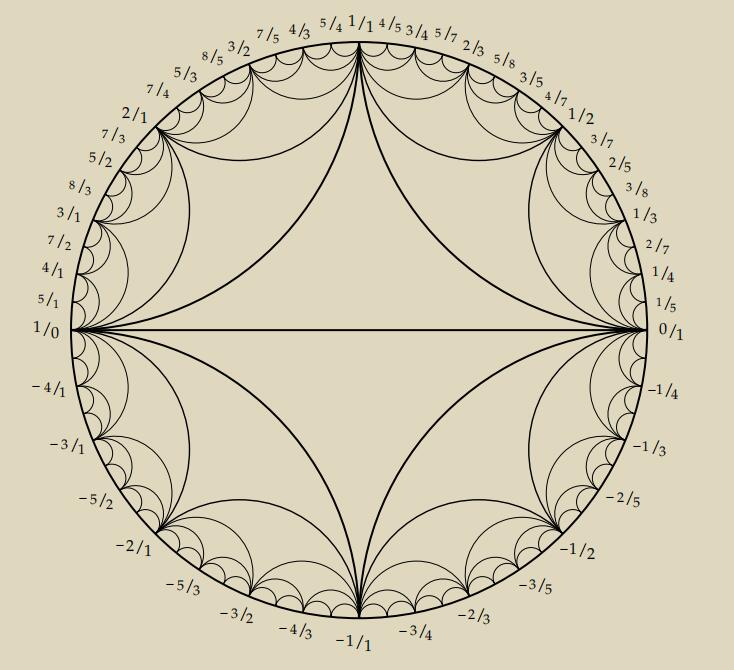
\includegraphics[scale=0.5]{FareyDiagram.jpg}
    \caption{Farey Graph}
    \label{FareyDiagram}
\end{figure}
\par
The diagram has infinitely many curvilinear triangles, getting smaller and smaller out near the boundary circle. The diagram can be constructed by first inscribing the two big
triangles in the circle, then adding the four triangles that share an edge with the two
big triangles, then the eight triangles sharing an edge with these four, then sixteen
more triangles, and so on forever. Our first task will be to explain how the vertices of all the
triangles are labeled with rational numbers.
\par
The vertices of the triangles in the Farey graph are labeled with fractions a/b,
including the fraction 1/0 for $\infty$, according to the following scheme. In the upper
half of the diagram first label the vertices of the big triangle 1/0, 0/1, and 1/1. Then one inserts labels for successively
\par
smaller triangles by the rule that, if the labels at the two ends
of the long edge of a triangle are a/b and c/d, then the label
on the third vertex of the triangle is $\frac{a+c}{b+d}$
. This fraction is called the mediant of a/b and c/d.
\par
The labels in the lower half of the diagram follow the same scheme, starting with
the labels 1/0, 0/1, and 1/1 on the large triangle. Using 1/0 instead of 1/0 as
the label of the vertex at the far left means that we are regarding $+\infty$ and $-\infty$ as the
same. The labels in the lower half of the diagram are the negatives of those in the
upper half, and the labels in the left half are the reciprocals of those in the right half.
\par
Our usual custom will be to write fractions with a positive denominator, so the
sign of the fraction is the sign of the numerator. This rule does not apply to the
ambiguous fraction $1/0 = -1/0$, of course.
\par
With a construction like this it is not easy to tell by a simple calculation whether or not two given rational numbers a/b and c/d are joined by an edge in the diagram. Fortunately there is such a criterion:
\begin{proposition}
\label{prop3.1}
For each pair of fractions $a/b$ and $c / d$, including $\pm 1 / 0$, there exists an edge in the Farey graph with endpoints labeled $a / b$ and $c / d$ if and only if the determinant $ad-bc$ of the matrix $\left(\begin{array}{ll}a&c \\ b&d\end{array}\right)$ is equal to $1$ or $-1$.
\end{proposition}
\begin{proof}
Using induction and the idea of Euclidean Algorithm we can prove it. Details are seen in \cite{hatcher2002topology}.
\end{proof}
\begin{corollary}
The mediant rule for labeling the vertices in the Farey graph always
produces labels $a / b$ that are fractions in lowest terms.
\end{corollary}
\begin{proof}
Consider an edge joining a vertex labeled $a / b$ to another vertex labeled $c / d$ From the preceding proposition we have $a d-b c=\pm 1 .$ This implies that $a$ and $b$ are coprime since any common divisor of $a$ and $b$ must divide the products ad and $b c,$ hence also the difference $a d-b c=\pm 1,$ but the only divisors of $\pm1$ are $\pm1$
\end{proof}
The preceding proposition can also be used to prove another basic fact about the
Farey graph:
\begin{proposition}
 Every fraction $a/b$ in lowest terms occurs as the label on some vertex in the Farey graph.
\end{proposition}
\begin{proof}
Still be the process of Euclidean Algorithm.
\end{proof}
Once we have the Farey graph, we can construct the \textit{Farey complex}. In our picture of the Farey graph, we can see lots of boundaries of triangles: triples of vertices that are pairwise connected by an edge. We can imagine gluing in (two-dimensional) triangles in all of those places (this can be done formally using the notion of a quotient space). The Farey complex is the space obtained by gluing in all possible triangles to the Farey graph. From the definition we saw that every edge of the Farey graph is contained in exactly two triangles.
\par
Finally, we can define the\textit{ Farey tree}. The set of vertices is the
union of the set of edges of the Farey complex and the set of triangles of the Farey
complex. We connect two vertices when there is a containment relation. In other
words, when an edge of the Farey complex is contained in a triangle of the Farey complex, we connect the corresponding vertices of the Farey tree. Because of the
way we defined the Farey tree, we can visualize it as being superimposed on the
Farey complex; see Figure \ref{FareyTree}. Just to emphasize: there are two types of vertices of the Farey tree—corresponding to edges and to triangles of the Farey complex—and
adjacent vertices have different types. 
\par
The Farey tree is indeed a tree according to our definition of Farey graph
\begin{figure}
    \centering
    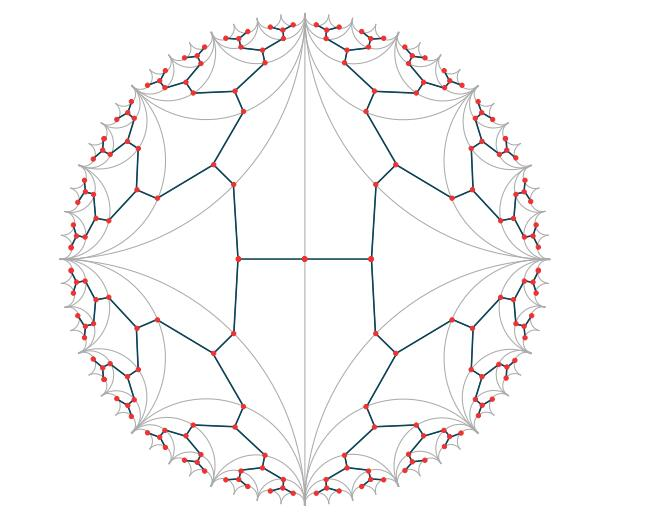
\includegraphics[scale=0.5]{FareyTree.jpg}
    \caption{The Farey tree superimposed on the Farey complex.}
    \label{FareyTree}
\end{figure}


\subsection{$SL_2(\mathbb{Z})$-action on the Farey tree}
\label{chap4.2}
For a fraction $a/b$ in lowest terms labeling on a point of the Farey Tree, we can equivalently write it as a representative $\pm(a,b)$. In this way we obtain an action of $SL_2(\mathbb{Z})$ on Farey graph by matrix multiplication (It is easy to check that the action on vertices preserves adjacency and non-adjacency  of vertices with help from proposition \ref{prop3.1}. Also, the action of $SL_2(\mathbb{Z})$ on the Farey graph induces an action on the Farey complex, meaning that the action on the graph takes the boundary of a triangle to the boundary of a triangle: Let $A\in SL_2(\mathbb{Z})$, then
$A\left(\begin{array}{lll}
p&r&p+r \\
q&s&q+s
\end{array}\right)$
preserves the graph relations of the three points $\pm(p,q),\pm(r,s),\pm(p+r,q+s)$. Again, the action of $SL_2(\mathbb{Z})$ on the Farey complex carries over to an action on the Farey tree.
\par
Now we study the properties of this action.
\\
\\
\noindent
\textit{No inversions.} Since the action of $SL_2(\mathbb{Z})$ on the Farey complex cannot interchange an edge and a triangle, the action of $SL_2(\mathbb{Z})$ on the Farey tree cannot interchange vertices of two different types. In other words, $SL_2(\mathbb{Z})$ acts on the Farey tree without inversions.
\\
\\
\noindent
\textit{Stabilizers of vertices corresponding to edges of the Farey complex.} Let us first deal with the vertex $v$ of the Farey tree corresponding to the edge of the Farey complex connecting the vertices $\pm(1,0)$ and $\pm(0,1) .$ For an element of $SL_2(\mathbb{Z})$ to stabilize
$v,$ it simply must preserve the set
\[
\{(1,0),(-1,0),(0,1),(0,-1)\}
\]
Now, the columns of a matrix are just the images of the standard basis vectors under the action of that matrix. Therefore, the columns of our stabilizer must lie in this list of four elements. That gives exactly $\left(\begin{array}{l}4 \\ 2\end{array}\right)=6$ matrices to think about. But we cannot choose a vector and its negative, for then the determinant will be 0. It turns out that the other four matrices all have determinant 1:
\[
\left(\begin{array}{ll}
1 & 0 \\
0 & 1
\end{array}\right),\left(\begin{array}{rr}
0 & 1 \\
-1 & 0
\end{array}\right),\left(\begin{array}{rr}
-1 & 0 \\
0 & -1
\end{array}\right),\left(\begin{array}{rr}
0 & -1 \\
1 & 0
\end{array}\right)
\]
These are exactly the elements of the cyclic group generated by the second matrix on the list. So the stabilizer of $v$ is a cyclic group of order 4.
\\
\\
\noindent
\textit{Stabilizers of vertices corresponding to triangles of the Farey complex. }As in the
last case, it suffices to consider the case of the vertex corresponding to the triple
\[
\pm(1,0) \quad \pm(0,1) \quad \pm(1,1)
\]
(prove the analogous claim). If an element of $SL_2(\mathbb{Z})$ fixes this vertex of the Farey tree, it must take (1,0) to one of the six vectors listed and it must take (0,1) to another one of the six vectors. But the images of these vectors are the columns of the given element of $SL_2(\mathbb{Z}),$ and so there are only a few possibilities for the stabilizer of this vertex in $SL_2(\mathbb{Z}),$ namely, the matrices
\[
\left(\begin{array}{ll}
1 & 0 \\
0 & 1
\end{array}\right),\left(\begin{array}{rr}
0 & 1 \\
-1 & 1
\end{array}\right),\left(\begin{array}{ll}
-1 & 1 \\
-1 & 0
\end{array}\right)
\]
and their negatives.
\\
\\
\noindent
\textit{Transitivity on the vertices of the Farey tree corresponding to edges of the Farey complex.} Take the vertex $v$ of the Farey tree corresponding to $\{\pm(p, q), \pm(r, s)\} .$ We will show there is an element of $SL_2(\mathbb{Z})$ taking the standard vertex $v_{0}$ given by $\{\pm(1,0), \pm(0,1)\}$ to $v .$ By the definition of the Farey tree, the determinant of
\[
\left(\begin{array}{ll}
p & r \\
q & s
\end{array}\right)
\]
is 1 (after possibly replacing $(r, s)$ with $-(r, s)$ ). But then this is the matrix we were looking for!
\\
\\
\noindent
\textit{Transitivity on the edges of the Farey tree.} Recall that an edge of the Farey tree connects one vertex corresponding to an edge of the Farey complex to one vertex corresponding to a triangle of the Farey complex. We have a favorite edge $e_{0},$ namely the one connecting the vertex $v_{0}$ corresponding to $\{\pm(1,0), \pm(0,1)\}$ to the vertex $w_{0}$ corresponding to $\{\pm(1,0), \pm(0,1), \pm(1,1)\} .$ We will show that we can take any other edge to this one using an element of $SL_2(\mathbb{Z})$.
\par
Consider an edge $e$ connecting vertices $v$ and $w$ of the Farey tree. And say that $v$ corresponds to $\{\pm(a, b), \pm(c, d)\} .$ The fact that $\pm(a, b)$ and $\pm(c, d)$ span an edge of the Farey complex means that one of the matrices
\[
A=\left(\begin{array}{ll}
a & c \\
b & d
\end{array}\right) \quad \text { or } \quad A^{\prime}=\left(\begin{array}{cc}
a & -c \\
b & -d
\end{array}\right)
\]
has determinant $1 ;$ say $A$ does. Then $A^{-1} v=v_{0} .$ We are halfway there-we just need to find a matrix $B$ that stabilizes $v_{0}$ and takes $w_{0}$ to $A^{-1} w .$ Then $B^{-1} A^{-1} e$ will be equal to $e_{0},$ as we wanted.
\par
So what is $A^{-1} w ?$ All we know is that it is some vertex of the Farey tree that is connected to $v_{0} .$ Well, there are only two of those, since an edge of the Farey complex is contained in exactly two triangles. There is $w_{0},$ and the vertex corresponding to $\{\pm(1,0), \pm(0,1), \pm(1,-1)\} ;$ call it $w_{1} .$ If $A^{-1} w=w_{0}$ there is nothing to do. But there is the possibility that $A^{-1} w=w_{1},$ and so we need to show that there is a matrix $B$ in $SL_2(\mathbb{Z})$ taking $w_{0}$ to $w_{1}$ (in other words, we are showing that the stabilizer of $v_{0}$ acts transitively on the vertices adjacent to $v_{0}$ ).
\par
Remember that we already computed the stabilizer of $v_{0}$ earlier. It is the group of matrices consisting of
\[
\left(\begin{array}{ll}
1 & 0 \\
0 & 1
\end{array}\right),\left(\begin{array}{rr}
0 & 1 \\
-1 & 0
\end{array}\right)
\]
and their negatives. But the second matrix takes the vertex $w_{0}$ to $w_{1},$ and so we have succeeded in showing that $SL_2(\mathbb{Z})$ acts transitively on the edges of the Farey tree.
\\
\\
\noindent
\textit{Stabilizers of edges} If an element of $SL_2(\mathbb{Z})$ fixes the edge $e_{0}$ we were just looking at, then it must lie in the intersection of the stabilizers of $v_{0}$ and $w_{0} .$ But this intersection is just the identity matrix and its negative.
\\
\\
After all the preparing work, we can now write down our presentation for $SL_2(\mathbb{Z})$. The hard part is already done: $SL_2(\mathbb{Z})$ acts without inversions on the Farey tree and that it acts transitively on edges, and we have already computed the stabilizers of $e_{0}, v_{0},$ and $w_{0}:$ they are isomorphic to $\mathbb{Z} / 2 \mathbb{Z}, \mathbb{Z} / 4 \mathbb{Z}$ and $\mathbb{Z} / 6 \mathbb{Z}$. Therefore, applying the theorem \ref{thm3.3}, we have the following isomorphism
\begin{theorem}
\label{thmain}
The group $SL_2(\mathbb{Z})$ can be presented as
\[
S L_{2}(\mathbb{Z}) \cong \mathbb{Z} / 4 *_{\mathbb{Z} / 2} \mathbb{Z} / 6
\]
where the subgroups $\mathbb{Z} / 2, \mathbb{Z} / 4, \mathbb{Z} / 6$ are generated by
\[
\left(\begin{array}{rr}
-1 & 0 \\
0 & -1
\end{array}\right),\left(\begin{array}{cc}
0 & 1 \\
-1 & 0
\end{array}\right),\left(\begin{array}{rr}
0 & -1 \\
1 & 1
\end{array}\right)
\]
respectively and the gluing maps $\mathbb{Z} / 2\hookrightarrow\mathbb{Z} /4$ and $\mathbb{Z} / 2\hookrightarrow\mathbb{Z} /6$ are inclusions.
\end{theorem}

\subsection{The Homology of $SL_2(\mathbb{Z})$}
Now we can calculate the homology of the linear group, $SL_2(\mathbb{Z})$.
\par
We proved the theorem \ref{thmain} in last section:
\[
S L_{2}(\mathbb{Z}) \cong \mathbb{Z} / 4 *_{\mathbb{Z} / 2} \mathbb{Z} / 6
\]
\par
Now consider the map $S L_{2}(\mathbb{Z}) \rightarrow \mathbb{Z} / 12$ defined by sending the generator of $\mathbb{Z} / 4$ to 3 mod 12 and the generator of $\mathbb{Z} / 6$ to 2 mod 12
\begin{theorem}
\label{thm3}
The $\operatorname{map} S L_{2}(\mathbb{Z}) \longrightarrow \mathbb{Z} / 12$ induces an isomorphism in integral homology:
\[
H_{i}\left(S L_{2}(\mathbb{Z}), \mathbb{Z}\right) \cong H_{i}(\mathbb{Z} / 12, \mathbb{Z}) \cong\left\{\begin{array}{ll}
\mathbb{Z} & i=0 \\
\mathbb{Z} / 12 & i \text { odd } \\
0 & i \text { even }
\end{array}\right.
\]
\end{theorem}
\begin{proof}
Associated to any decomposition $G=G_{1} *_{A} G_{2},$ there is a Mayer-Vietoris sequence as to corollary \ref{cor1}
\[
\cdots \rightarrow H_{i}(A) \rightarrow H_{i}\left(G_{1}\right) \oplus H_{i}\left(G_{2}\right) \rightarrow H_{i}(G) \rightarrow H_{i-1}(A) \rightarrow \cdots
\]
The homology of a cyclic group $\mathbb{Z} / n$ is given by example \ref{example1}
\[
H_{i}(\mathbb{Z} / n, \mathbb{Z})=\left\{\begin{array}{ll}
\mathbb{Z} & i=0 \\
\mathbb{Z} / n & i \text { odd } \\
0 & i \text { even }
\end{array}\right.
\]
Moreover, it is easy to see that if $\mathbb{Z} / n \rightarrow \mathbb{Z} /(n m)$ is the inclusion $1 \mapsto m,$ then the map $H_{2 i-1}(\mathbb{Z} / n) \rightarrow H_{2 i-1}(\mathbb{Z} /(n m))$ is the same inclusion that maps the identity 1 in the torsion part $\mathbb{Z} / n$ to m in $\mathbb{Z} / (n m)$. For example, in the following figure \ref{fig:my_label} we calculate the case $\mathbb{Z} / 2\hookrightarrow\mathbb{Z} /4$.
\begin{figure}
    \centering
    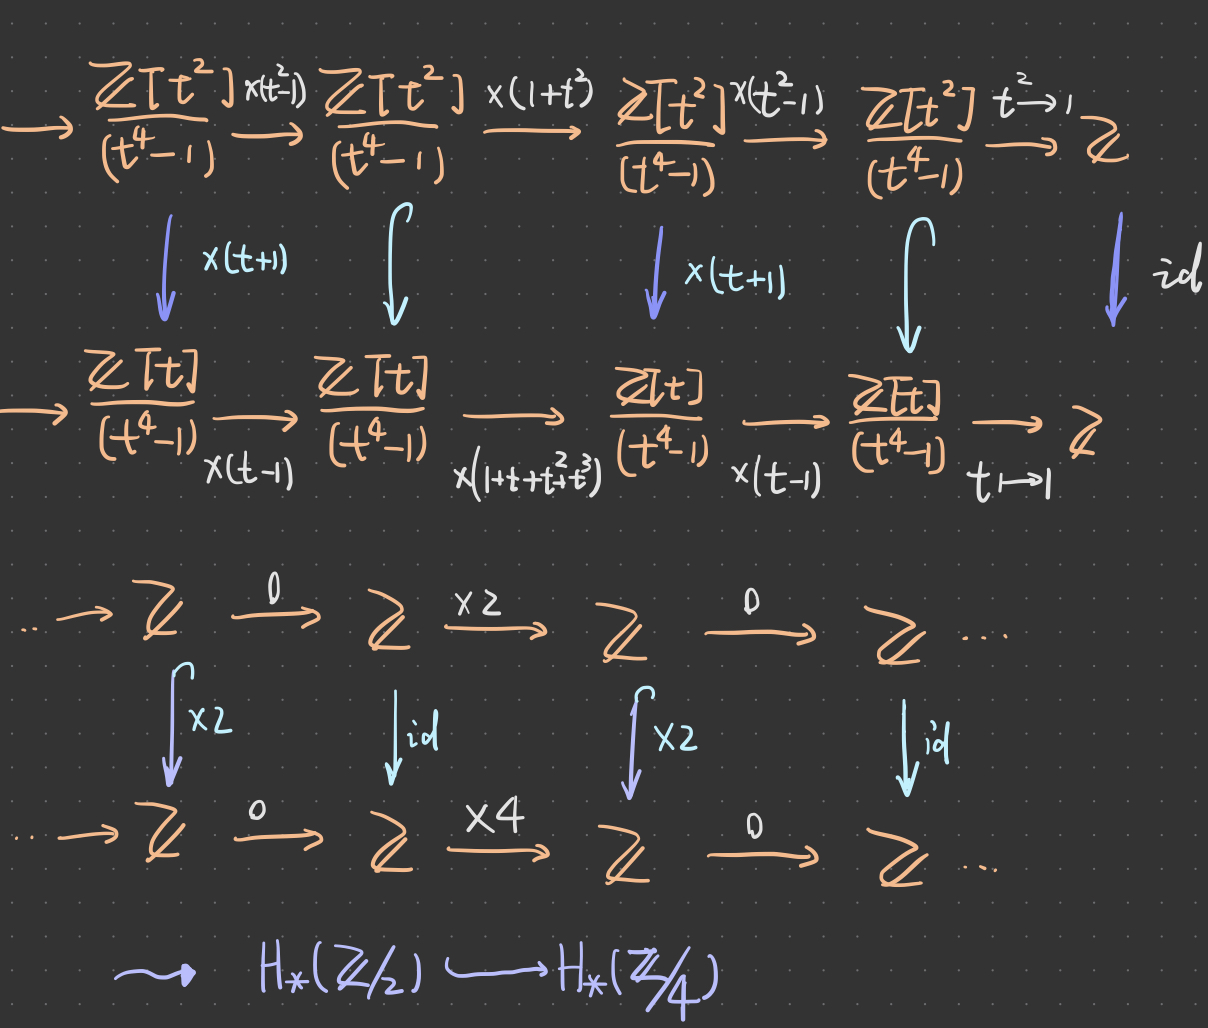
\includegraphics[scale=0.2]{injection.jpg}
    \caption{$\mathbb{Z} / 2\hookrightarrow\mathbb{Z} /4$}
    \label{fig:my_label}
\end{figure}
\newpage
It follows that the sequence for computing $H .\left(S L_{2}(\mathbb{Z})\right)$ has the following form:
\[
0 \rightarrow H_{2 i}\left(S L_{2}(\mathbb{Z})\right) \rightarrow \mathbb{Z} / 2 \rightarrow \mathbb{Z} / 4 \oplus \mathbb{Z} / 6 \rightarrow H_{2 i-1}\left(S L_{2}(\mathbb{Z})\right) \rightarrow 0
\]
$\operatorname{since} H_{2 i}(\mathbb{Z} / n)=0$ for all $n, i \geq 1 .$ Note that the $\operatorname{map} \mathbb{Z} / 2 \rightarrow \mathbb{Z} / 4 \oplus \mathbb{Z} / 6$ is
injective so that $H_{2 i}\left(S L_{2}(\mathbb{Z})\right)=0$ for $i \geq 1$ and $H_{2 i-1}\left(S L_{2}(\mathbb{Z})\right)$ has order 12 One checks easily that $H_{2 i-1}\left(S L_{2}(\mathbb{Z})\right)$ is in fact cyclic with generator $(1,2)$ .
\end{proof}

\begin{remark}
For other arithmetic linear groups, like the cohomology of $SL_2(\mathbb{Z}[1/p])$ for p prime, it was completely calculated by A. Adem and M. Naffah in \cite{adem1998cohomology}. The homology of $SL_2(\mathbb{Z}[1/m])$ for small m can be computed using a kind of algorithm introduced in \cite{bui2014homology}. For further information on the homology of $SL_2(R)$ for R being one dimensional ring, one can refer to Chapter.4 of \cite{knudson2012homology} and its Chapter.5 for further application of these results.
\end{remark}


%\section{Homology of Other Rank One Groups}
\appendix
\section{Basic Bricks of the Trade}
This appendix is written here for the completeness of the proof of lemma \ref{lemma3}.
\par
In homotopy theory every map $f: A \rightarrow B$ from a space $A$ to a pathconnected space $B$ may be viewed as either an inclusion or a fibering. We can see this as follows.
\subsection{Inclusion} 
\label{inc}
Applying the telescoping idea just once, we construct the mapping cylinder of $f$:

\begin{figure}[h!]
\centering
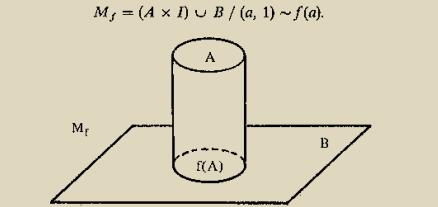
\includegraphics[scale=1]{mappingcylinder.jpg}
\caption{mapping cylinder}
\label{UN}
\end{figure}
It is clear that the mapping cyinder $M_{f}$ has the same homotopy type as $B$ and that $A$ is included in $M_{f}$. Indeed the following diagram is commutative:
$$
\xymatrix{
A \ar[d]^{id} \ar[r]^f &B\ar@{^{(}->}[d]^{\text{homotopy equivalence}}\\
A\ar@{^{(}->}[r] & M_f}
$$
\subsection{Fibering}
Let $f: A \rightarrow B$ be any map, with $B$ path connected. By section \ref{inc} we may assume that $f$ is an inclusion, i.e., $A$ is a subspace of $B$. Define
$L$ to be the space of all paths in $B$ with initial point in $A$. By shrinking every path to its initial point, we get a homotopy equivalence
\[
L \simeq A
\]
On the other hand by projecting every path to its endpoint, we get a fibering
\[
\begin{array}{c}
\Omega_{*}^{A}-L_{*} A \\
\downarrow_{ } \\
B
\end{array}
\]
$$\xymatrix{
\Omega_{*}^{A}\ar[r]& L \ar[d]\\
&B
}$$
Whose fiber is $\Omega_{*}^{A},$ the space of all paths from a point $*$ in $B$ to $A .$ So up to homotopy equivalence, $f: A \rightarrow B$ is a fibering.

\bibliographystyle{plain}
\bibliography{references}
\end{document}
